\section{Related work}
\begin{figure*}[htbp]
	\centering
	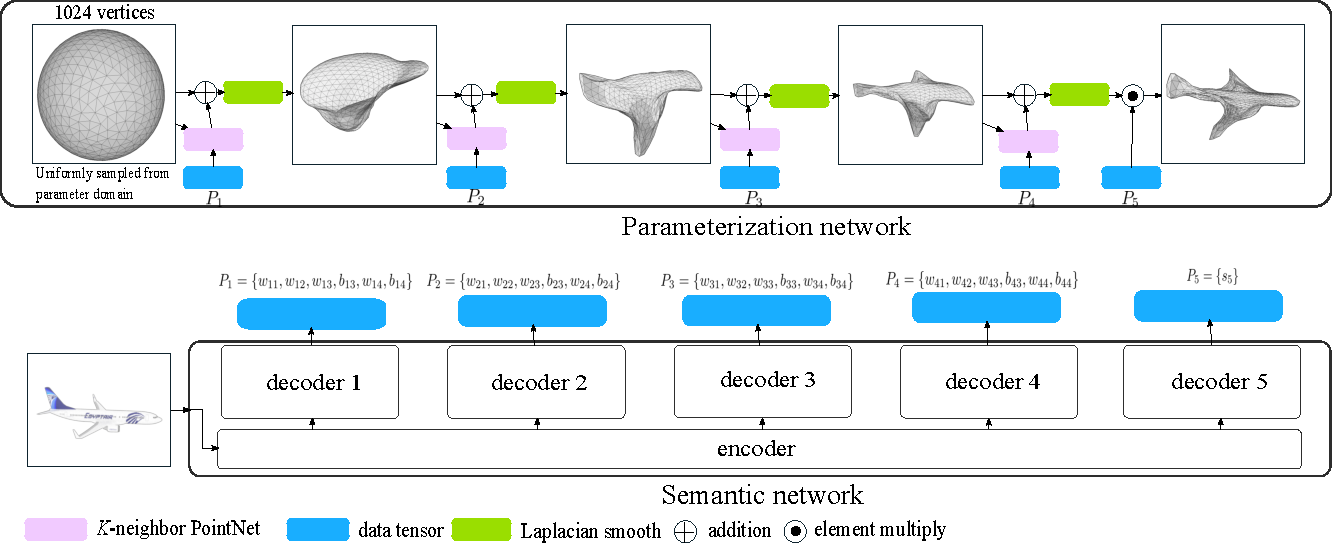
\includegraphics[width=\linewidth]{img/net/overview}
	\caption{The overview of the network: The proposed framework consists of two networks. One is the parameterization network that maps points sampled from parameter domain to target shape. The other is the semantic network that takes image as input and predict parameters for the parameterization network. \cxj{Merge semantic network and parameterization network.}}
	\label{fig:overview}
\end{figure*}

3D reconstruction and modeling from a single image has been extensively studied as the problem of \emph{shape from monocular cues}, including shadings~\cite{shapefromshadingsurvey}, focuses~\cite{shapefromdf1,shapefromdf2}, and textures~\cite{Aloimonos1988}. 
These methods usually recover 2.5D surfaces from 2D images. 
Learning-based approaches, especially deep learning methods, can acquire more complicate priors by learning from datasets and recover much more complete 3D shape from a single image.
 
\subsection{General learning approaches}
As far as we known, early work of learning approaches can be traced back to \cite{Hoiem2007} and \cite{learn3D2007}. \cxj{explain them in one or two sentences.}
%
More recent techniques break down the problem to two stages\cite{Su:2014,jointimgshape}. One is to retrieve shape components from a large dataset, and the other is to assemble the components and deform the assembled shape to fit the observed image. 
%
However, shape retrieval from images itself is an challenging problem due to the loss of information during 3D-to-2D projection. 
\cite{imgrecon15} proposes a solution that starts reconstruction from a learned 3D deformable shape. 
In \cite{imgrecon15}, images specify the shape variations and drive the shape deformation to target.
\cxj{confusing..}
%
%These learning approaches are relatively early.
In these methods, complicated pre-processing on the databases are usually needed.
\cxj{Like what?} 
%A more ideal solution would be to directly learn 3D shapes from single images under an end-to-end framework. 

\begin{figure*}[htbp]
	\centering
	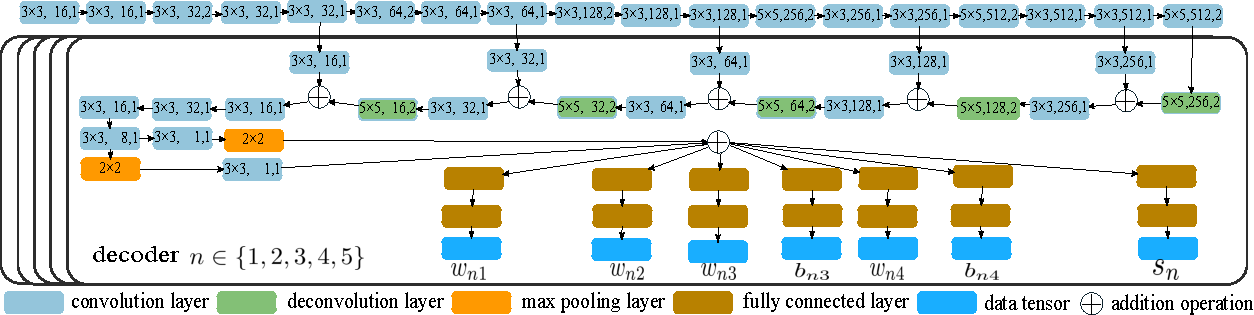
\includegraphics[width=\linewidth]{img/net/semnet}
	\caption{Semantic network: The semantic network takes image as input and predict parameters for the \textit{K}-neighbor PointNet and the global scale operation in the parameterization network. The semantic network have separate decoders for each \textit{K}-neighbor PointNet and and the global scale operation. }
	\label{fig:semnet}
\end{figure*}

\subsection{3D neural networks}
Most recently, researchers have developed techniques to represent 3D shapes inside deep learning frameworks.%, and developed a serious of 3D neural networks to predict 3D shapes from images. 
Unlike images, 3D shapes are not canonical functions \mdf{on well-organized grids}. 
This leads to exploration on various representations of 3D shapes.

\noindent\textbf{Volume occupancy.} 
An intuitive way to apply convolutional network in 3D is to use volume occupancy of regular 3D grids to represent 3D shapes~\cite{3dshapenet}, and it is subsequently use for 3D shape generation~\cite{3DR2N2,learnobj}.
%
The main disadvantage of volumetric representation was the large memory consumption due to the raising of dimension when extending 2D grids to 3D. 
Octree representation is proposed to support higher resolution outputs with limited memory, and used for shape generation~\cite{octreegen} and shape classification~\cite{ocnn}.
%The most recent work of use an octree representation for shape generation (similar representation is used in for 3D shape classification and segmentation by \cite{ocnn}), which allows to higher resolution outputswith limited memory.

\noindent\textbf{Point clouds.} 
Compared to regular 3D grids, point clouds do not carry local connections between points. 
Many networks have been proposed to take unordered 3D point sets as input and extract geometric features from 3D point set for classification or segmentation~\cite{PointNet,NIPS2017_7095,pointcnn}.
%
The \cxj{first attempt?} was made to generate a set of discrete points from a single image using neural networks~\cite{PSGN}, however, it is non-trivial to construct continuous surface models from the predicted point sets. \cxj{because of what? various density and thinknesses?}



\comments{
\cite{PSGN} proposed neural networks that regress unordered
3D point set for 3D shape generation. The point cloud representation
do not consider local connections of the points, and thus the point positions have
a very large degree of freedom. Consequently, it is difficult to reconstruct continue surface from the generated point cloud.}


\noindent\textbf{Meshes}
%Among all three representations, 
Meshes are widely used in game and movie industries. 
In addition to vertex positions, the mesh representation contains local structure of vertices. 
However, the mesh representation is not well supported in current neural networks.
% 
To generate mesh models by using neural networks, composition weights of a series of base meshes are predicted by networks~\cite{img2mesh} and \cite{endface}. %produce meshes by linear interpolating base meshes. 
Since it is only possible to choose/learn base meshes for specific class of object, these two networks only generates meshes for a specific class of object, such as face.
%(the latter one is only used for human face).
%
\cite{3Drender} aims to make a differentiable approximation for 3D mesh rendering process, which would be much more significant if it could render gray image. 
In fact, the approximated renderer can only produce silhouettes as output. 
When it is used for mesh generation, it only take silhouette as supervision, hence does not perform well for complicated objects, such as cars, airplanes, etc.
%
In comparison, our network draws a lot of experiences from techniques designed for point cloud representation, and it directly produces meshes as output.
%but it .

\subsection{Parameterization in Learning.}
The idea of utilizing surface parameterization in neural networks has been explored\cite{surfnet,geoimg}. 
Typically, a non-trainable procedure is involved for the creation of geometry image. 
Manifold surfaces are required as training data so that the shapes can be parameterized using spherical parameterization and turned into geometry image. However, the public datasets like ShapeNet\cite{shapenetdata} contain meshes that are not manifold surfaces. 
In comparison, we represent 3D surfaces by surface parameterization. 
Our proposed network predicts a mapping from the parameter domain to the target surface. Manifold surfaces are not necessary as supervision.
Out network can be trained with point clouds as supervision, but it directly produces mesh models.
